\documentclass[sigconf]{acmart}
% The preceding line is only needed to identify funding in the first footnote. If that is unneeded, please comment it out.
% On windows run updmap
\usepackage[utf8x]{inputenc}
\usepackage{amsmath,amsfonts}
\usepackage{algorithmic}
\usepackage{graphicx}
\usepackage{textcomp}
\usepackage{listings}
\usepackage{xcolor}
\usepackage{multirow}
\usepackage{dcolumn}
\usepackage{booktabs} 
\usepackage{pifont}  % use /ding{55} for X... /ding{51} for check
\usepackage{url}
\usepackage{hyperref}
\usepackage{adjustbox}
\usepackage{threeparttable}
\usepackage{xspace}
\usepackage{placeins}
\usepackage[nameinlink]{cleveref}

\expandafter\newcommand\csname r@tocindent4\endcsname{4in}
\setcounter{secnumdepth}{4}
\setcounter{tocdepth}{4}

\lstset{
language=Java,
basicstyle=\small\ttfamily,			
keywordstyle=\color{blue},
commentstyle=\color{gray},			
stringstyle=\color{black},					
}


\AtBeginDocument{%
  \providecommand\BibTeX{{%
    \normalfont B\kern-0.5em{\scshape i\kern-0.25em b}\kern-0.8em\TeX}}}

% My 'newcommand' for modulo function...
\newcommand{\abs}[1]{\left|#1\right|}


% My 'newcommand' for standard table creation...
\newcommand{\AndreaTable}[3]{\begin{table*}[h!]
\caption{#1}
\centering
\begin{tabular}{#2}
\toprule
#3
\bottomrule
\end{tabular}
\end{table*}
}

% My 'newcommand' for standard table creation...
\newcommand{\equivalenceClassesTable}[2]{
\AndreaTable{#1}{llm{8cm}m{8cm}}{#2}
}


\definecolor{beaublue}{rgb}{0.74, 0.83, 0.9}


\settopmatter{printacmref=false, printccs=false, printfolios =false}
\setcopyright{none} 
\renewcommand\footnotetextcopyrightpermission[1]{}
\acmConference[ISW2 Project A.A. 2019-2020]{ }{September 1, 2020}{ }

\begin{document}

\title{ISW2 Project A.A. 2019-2020}

\author{Andrea Graziani ($0273395$)}
\email{andrea.graziani93@outlook.it}
\affiliation{
  \institution{Università degli Studi di Roma "Tor Vergata"}
  \city{Rome}
  \country{Italy}
}

\keywords{Testing, Equivalence Class Partitioning, Boundary Value Analysis, Mutation Testing}
\maketitle

\section{Deliverable 2}

\subsection{Introduction}

How to detect software modules which are more \textbf{defect-prone} than others? Why we are interested to identify them? 

These are some of the most critical questions of software engineering, to which we will try to answer. 

Firstly, a \textbf{software defect} can be generally considered as an error, flaw, bug, mistake, failure, or fault in a computer program or system that may generate an inaccurate or unexpected outcome, or precludes the software from behaving as intended \cite{SoftwareDefectPredictionRawat}.

As known, the presence of defective software modules \textit{always incurs cost in terms of time and money}, because identifying and rectifying defects is one of the most time consuming and expensive software processes \cite{SoftwareDefectPredictionRawat}.

Although it's not practically possible to eliminate each and every defect from a software product, we can reduce their adverse effects exploiting \textbf{software defects prediction} techniques, \textit{which aim is to identify software modules that are defect-prone, in order to reduce the cost of testing activities and code review by letting developers focus on specific artefacts} \citep{Falessi}.

How to build a software defect prediction model? 

In this report, we will describe a software defect prediction model based on \textbf{machine learning} techniques, which building passes through following steps:

\begin{itemize}
\item \textbf{Dataset building}.
\item \textbf{Dataset labelling}.
\item \textbf{Preprocessing}.
\end{itemize}


\subsection{Dataset building}

The first step is, obviously, to \textbf{generate a data-set}, in order to provide an appropriate input for our prediction model; in other words, we need to build a set of \textbf{instances}. 

In our context, each data-set's instance represents a \textbf{source code file} belonging to one of the following open-source software projects which we have analysed:

\begin{description}
\item[Apache BookKeeper\texttrademark]Which is a scalable, fault tolerant and low latency storage service\footnote{\url{https://github.com/apache/bookkeeper}}.
\item[Apache OpenJPA\texttrademark]An implementation of the Java Persistence API specification\footnote{\url{https://github.com/apache/openjpa}}. 
\end{description}

Every data-set's instance is characterized by its values on a fixed, predefined set of \textbf{features}, or \textbf{attributes}, like its code lines number, its age, its complexity and so on. Clearly, in order to build an useful software predictor, \textit{is preferable to collect instances whose features are correlated to the defect-proneness of the software module they belong}. Fortunately, scientific literature reports many studies, about software defect-proneness, which had identified several features (sometimes called also \textbf{metrics}) correlated with defect density of a software module. 

For example, \citet{PredictingDefectsForEclipse} showed that the number of past defects has the highest correlation with number of future defects. \citet{Nagappan} report that \textit{code churn} is a very powerful metric for predict software defect density, while \citet{Gyimothy} showed the same with \textit{lines of code} (\texttt{LOC}) metric.

\subsubsection{Our implementation}
\hfill\\

We extracted these defect-proneness correlated features from \textit{history data} of our projects, exploiting tools like \texttt{git}\footnote{\url{https://git-scm.com/}}, the most famous \textit{version control systems} today available, and \texttt{JIRA}\footnote{\url{https://www.atlassian.com/it/software/jira}}, which is a \textit{issue tracking systems}.

From an implementation point of view, the \texttt{Git} class\footnote{Complete path: \texttt{datasetbuilder.datasources.vcs.git.Git}} contains the entire application logic to manage a \texttt{git} repository, implementing \texttt{Version\-Control\-System} interface, reported in \textbf{\cref{interface1}}). 

To be more precise, this class has following responsibilities: 
\begin{itemize}
\item To identify the commit associated to each project's release.
\item To extract metrics of a given source code file; this is done invoking \texttt{compute\-File\-Metrics} method.
\item To identify all source code files belonging to a release.
\end{itemize}

\begin{lstlisting}[frame=lines,basicstyle=\ttfamily\scriptsize, caption={\texttt{VersionControlSystem} interface}, label={interface1}]
public interface VersionControlSystem {

    Commit getCommitByTag(String tag);

    Commit getCommitByDate(LocalDateTime date);

    Commit getCommitByLogMessagePattern(String pattern);

    Map<String, File> getFiles(String commitHash);

    List<String> getFilesChangedByCommit(String commitHash);

    void computeFileMetrics(File file, Commit releaseCommit);
}
\end{lstlisting}

To be more precise, \texttt{compute\-File\-Metrics} method was been developed in order to extract all metrics reported and described in \textbf{\cref{metrics}}. 

\begin{table}
\caption{Metrics extracted from source code file $X$ by \texttt{compute\-File\-Metrics} method}
\label{metrics}
\begin{tabular}{l|p{4.3cm}}
\toprule
\textbf{Name} & \textbf{Description} \\
\midrule

\texttt{LOC} & Lines of code of $X$. 

\\

\texttt{LOC\_TOUCHED} & $\sum_R (\texttt{addedLOC} + \texttt{deletedLOC})$ \newline Where: 

\begin{itemize}
\item $R$ is the set of all revisions of $X$.
\item $\texttt{addedLOC}$ represents the number of added code lines.
\item $\texttt{deletedLOC}$ represents the number of removed code lines.
\end{itemize}

\\

\texttt{LOC\_ADDED} & $\sum_R (\texttt{addedLOC})$

\\

\texttt{MAX\_LOC\_ADDED} & $\max_R (\texttt{addedLOC})$.

\\
    
\texttt{AVERAGE\_LOC\_ADDED} & $\dfrac{\sum_R (\texttt{addedLOC})}{\mid R \mid}$

\\

\texttt{NUMBER\_OF\_REVISIONS} & $\mid R \mid$ 

\\

\texttt{NUMBER\_OF\_FIX} & Number of bug fixes which have involved $X$.

\\

\texttt{NUMBER\_OF\_AUTHORS} & The authors number which developed file $X$.

\\

\texttt{CHURN} & $\sum_R (\texttt{addedLOC} - \texttt{deletedLOC})$

\\

\texttt{MAX\_CHURN} & $\max_R (\texttt{addedLOC} - \texttt{deletedLOC})$

\\

\texttt{AVERAGE\_CHURN} & $\dfrac{\sum_R (\texttt{CHURN})}{\mid R \mid}$

\\

\texttt{MAX\_CHANGE\_SET\_SIZE} & The number of files committed together with $X$.

\\

\texttt{AVERAGE\_CHANGE\_SET\_SIZE} & $\dfrac{\texttt{MAX\_CHANGE\_SET\_SIZE}}{\mid R \mid}$

\\

\texttt{AGE\_IN\_WEEKS} & Age of $X$ in weeks.

\\

\texttt{WEIGHTED\_AGE\_IN\_WEEKS} & $\dfrac{\texttt{AGE\_IN\_WEEKS}}{\texttt{LOC\_TOUCHED}}$

\\

\bottomrule
\end{tabular}
\end{table}

\subsection{Dataset labelling}

To be precise, our aim is to build a software defect predictor using a \textbf{supervised learning scheme}.

When a supervised learning scheme is used, the goal of our predictor is \textit{to learn a function that maps an input to an output based on example input-output pairs}. In other word, each data-set instance $T$ is represented as a pair $(x_{d}, y)$ where $x_d$ is a $d$-dimensional input object while $y$ is a \textit{tag}, or a \textit{label}, representing the \textit{desired output value}. In this way, a supervised learning algorithm, analysing \textit{labelled training data}, can produce an inferred function, which can be used for mapping \textit{unlabelled data}.

Therefore, the second very important step to build our predictor is the so-called \textit{labelling} task, according to which one or more informative tags must be assigned to each unlabelled instance of a given dataset.

\subsubsection{Our implementation}
\hfill\\

In our context, to build a properly data-set, we need to label each instance as \textit{buggy} or \textit{not buggy}. 

First of all, it is necessary to identify all project's releases. 

\texttt{Jira} class\footnote{Complete path: \texttt{datasetbuilder.datasources.its.jira.Jira}} contains application logic used to query \texttt{Jira} servers on the cloud. It implements the \texttt{Issue\-Tracking\-System} interface, shown in \textbf{\cref{interface2}}, providing the implementations for following methods:

\begin{description}
\item[\texttt{getReleases}] Which is used to retrieve all necessary information about project's releases, including names, release dates and so on.
\item[\texttt{getIssuesRegistry}] Invoked to get all data about known issues 
\end{description}

\begin{lstlisting}[frame=lines,basicstyle=\ttfamily\scriptsize, caption={\texttt{IssueTrackingSystem} interface}, label={interface2}]
public interface IssueTrackingSystem {

    List<Release> getReleases(String projectName);

    IssueRegistry getIssuesRegistry(
    	String projectName, 
    	Map<Integer, Release> releasesByVersionID);
}
\end{lstlisting}

Querying \texttt{Jira} is not enough, because to proceed we need all commits associated to each release.

To do that, we have exploited \texttt{git} tags inside commits messages to identify the commit associated to each release. 

However, when sometimes \texttt{git} tags were not available, we have identified aforementioned commits exploiting \texttt{git\- log} command with \texttt{--before\- [date]} options. The application logic to do that, is contained into \texttt{Git} class.

At this point, knowing commit associated to each release, we are able to retrieve all source code files associated to each project's release, however we still have to label them.

To do that we need to discover all known project's issues and, to do that, we queried once again \texttt{Jira} to obtain the identifiers of all issues with type \texttt{"Bug"} and status \texttt{"Closed"} (or \texttt{"resolved"}). We remember that is possible to find the implementation of this query procedure inside \texttt{get\-Issues\-Registry} method into \texttt{Jira} class.

Finally, to label each source code file as buggy or not, we need to check if the release, which the file belongs to, is an "\textit{Affected Version}" (\textbf{AV}).

Is very important to precise that scientific literature reports that most of the projects have more than $25\%$ of defects whose issue report contained no information about affected versions. Moreover, the vast majority of all bugs ($51\%$) resulted in not having or having an unreliable AV. Therefore, if information about the AV for a bug is available in \texttt{Jira}, we considered the earliest AV in \texttt{Jira} to be the release that introduced the bug, otherwise we have adopted the so-called \textbf{proportion method}.

\paragraph{The dormant defects problem}
\hfill\\
Empirical results show that is very common that a defect is discovered several releases \textit{after} its introduction \citep{Falessi}. 

This fact implies that if we observe, today, the status of a source code file in its current version, it can be considered as defect-free while, in reality, this conclusion is \textit{not} true because it can contain \textit{undiscovered defects}.

In according to scientific literature, these undiscovered defects, commonly called "\textit{dormant defects}" too, can negatively impacts our classifier's accuracy. We call "\textit{snoring}" the "\textit{noise}" consisting of all source code file containing dormant defects \citep{Falessi}.

In order to remedy, literature suggest \textbf{to remove the most recent releases from a dataset}. In fact, since earlier releases likely contain more snoring classes than older releases, removing the most recent is possible to reduce the snoring effect improving our classifiers evaluations. Since scientific literature states that the first 50\% of releases are not heavily impacted by snoring \citep{Falessi}, for every analysed project, we have choose to remove from our dataset half of available releases. From an implementation point of view, this task is done executing \texttt{retrieve\-Releases\-Discarding\-HalfOfThem} method, which belongs to \texttt{Project\-Dataset\-Builder} class \footnote{Complete path: \texttt{datasetbuilder.ProjectDatasetBuilder}}.

\subsection{Preprocessing}

After generating our data-set with metrics and labels, we applied a preprocessing technique called \textbf{feature selection} or \textbf{attribute selection}.

As known, most machine learning algorithms are designed to learn which are the most appropriate attributes to use for making their decisions. For example, decision tree methods choose the most promising attribute to split on at each point and should never select irrelevant or unhelpful attributes \cite{FalessiDataMining}. Although, theoretically, having more attributes give us a more discriminating power, in practice, adding irrelevant attributes to a dataset, performances of machine learning systems degrades \cite{FalessiDataMining}. 

Therefore, using a feature selection technique, deleting unsuitable attributes, is possible to \textit{improve learning algorithms performances}. However, using specific data-sets, is possible that they \textit{may require extensive computations}, degrading overall performances \cite{FalessiDataMining}.

How to select relevant features?

Clearly, the best way to select relevant attributes is \textit{manually}, based on a deep understanding of the learning problem. However, fortunately, automatic methods exist too. 

For our analysis, we have adopted \textbf{Best-first} method. This scheme adopts a \textit{greedy approach} to select an attribute subset that is most likely to make better predictions. Its peculiarity it that it does not just terminate when the performance starts to drop but keeps a list of all attribute subsets evaluated so far, sorted in order of the performance measure, so that it can revisit an earlier configuration instead \cite{FalessiDataMining}. 

At this point, our aim is to evaluate the advantages deriving from using a feature selection technique as best-first. How to do that?

\subsubsection{How to evaluate classifier accuracy}
\hfill\\

According to project specifications, we have used following classifiers, which implementation is provided by \texttt{Weka}\footnote{\texttt{https://www.cs.waikato.ac.nz/ml/weka/}}, an open source machine learning software:
\begin{itemize}
\item \textbf{Random Forest}
\item \textbf{IBK}
\item \textbf{Naive Bayes}
\end{itemize}

Our classifier's accuracy evaluation method consists of measuring following parameter:

\begin{description}

\item[\textbf{Recall}] also known as \textbf{true positive rate}, measures correctly predicted buggy instances among all buggy instances:

\begin{equation}
\dfrac{TP}{TP + FN}
\end{equation}

\item[\textbf{Precision}] which tell us many times our classifier has correctly classified an instance as buggy:

\begin{equation}
\dfrac{TP}{TP + FP}
\end{equation}

\item[\textbf{AUC}] measures the area under the \textit{receiver operating characteristic} (\textbf{ROC}) curve, plotted using \textit{false positive rate} and \textit{true positive rate} together.

\item[\textbf{Kappa}] tell to us how many times our classifier was been more accurate than a dummy classifier:

\begin{equation}
\dfrac{\text{Accuracy of classifier} - \text{Accuracy of dummy classifier}}{1 - \text{Accuracy of dummy classifier}}
\end{equation}

\end{description}
\hfill\\
\subsubsection{Evaluation results}
\hfill\\

Comparing results derived by processing our data-sets using best-first technique with those processed without feature selection algorithms, we have noted that best-first method is capable to \textbf{improve the accuracy of specific classifiers}.
 
As you can observe from \textbf{\cref{BOOKKEEPER-FeatureSelection}}, using our BookKeeper™ dataset, when a Naive Bayes classifier is used, exploiting best-first method without any sampling scheme (which we will describe in next section), we have obtained following results:
\begin{itemize}
\item \textit{Recall} parameter increased by $27.72\%$, passing from a value equal to $0.440$ to $0.562$. 
\item \textit{Kappa} parameter increased by $40.22\%$, from $0.179$ to $0.251$. 
\item \textit{ROC} parameter increased by $2.47\%$, from $0.686$ to $0.703$.
\item \textit{Precision} parameter decrease by $1.94\%$, from $0.630$ to $0.618$.
\end{itemize}

Our results confirm that Naive Bayes classifier improves its accuracy when best-first method is used. 



\begin{figure*}[h!]
  \centering
  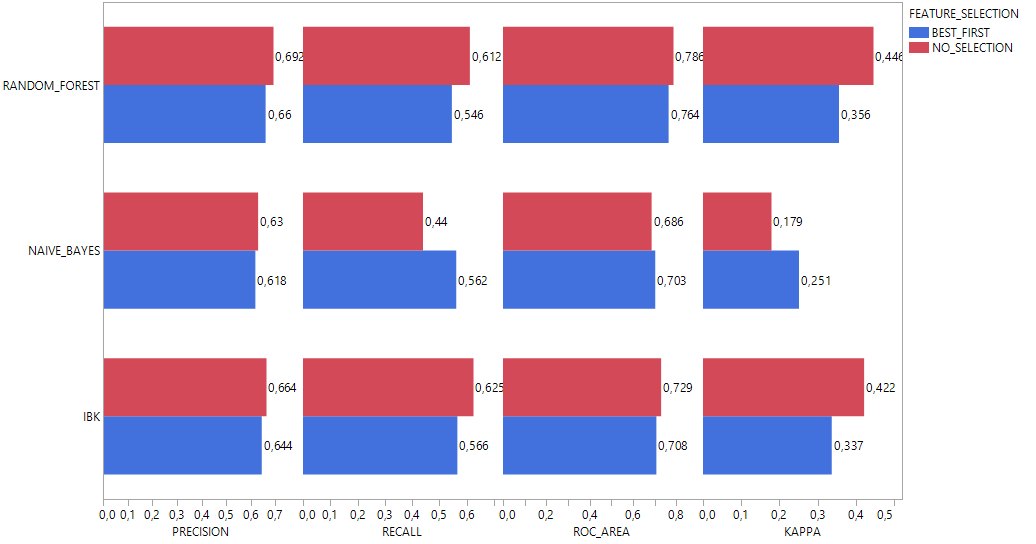
\includegraphics[width=\textwidth]{./BOOKKEEPER/FeatureSelection.png}
  \caption{Comparison of classifiers accuracy when using a feature selection algorithm. No sampling technique applied. BookKeeper™ project.}
  \label{BOOKKEEPER-FeatureSelection}
\end{figure*}

\begin{figure*}[h!]
  \centering
  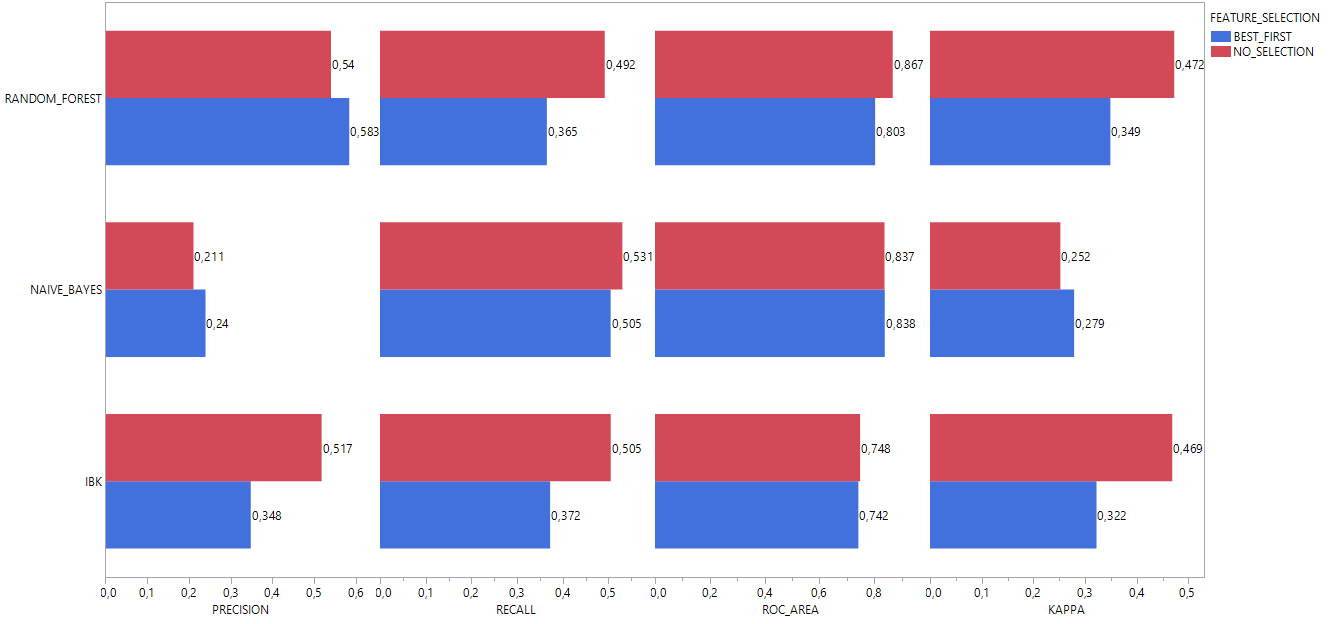
\includegraphics[width=\textwidth]{./OPENJPA/FeatureSelection.png}
  \caption{Comparison of classifiers accuracy when using a feature selection algorithm. No sampling technique applied. OpenJPA™ project.}
  \label{OPENJPA-FeatureSelection}
\end{figure*}

However, using others classifiers, we have obtained very different results. In fact, when random forest classifier is used, our experiment's results show that: 

\begin{itemize}
\item \textit{Recall} parameter decreased by $12,5\%$, passing from a value equal to $0.612$ to $0.544$. 
\item \textit{Kappa} parameter decreased by $25.28\%$, from $0.446$ to $0.356$. 
\item Both \textit{ROC} and \textit{Precision} parameters decreased by $2.87\%$ and $4.84\%$ respectively.
\end{itemize}

In other words, when Random Forest classifier is used, its accuracy get worse when best-first method is applied. IBK classifier shows results very similar to those of Random Forest. Using OpenJPA™ dataset, results are similar. 

\FloatBarrier

\subsection{Sampling}
\hfill\\

As known, performance of a software defect prediction model depends heavily on the data on which it was trained. In fact, defect prediction models that are trained on imbalanced datasets, that is datasets where the proportion of defective and clean modules is not equally represented, are highly susceptible to producing inaccurate prediction models \cite{FalessiSampling}

To mitigate the risk of imbalanced datasets during our analysis, we have adopt following class rebalancing techniques.

\begin{description}
\item[Over-sampling] It randomly samples with replacement the minority class to be the same size as the majority class. It is also known as up-sampling.

\item[Under-sampling] It samples the majority class in order to reduce the number of majority modules to be the same number as the minority class. It is also known as down-sampling.

\item[SMOTE] This technique combats the disadvantages of both over-sampling and under-sampling techniques, creating artificial data based on the feature space similarities from the minority class. 

\end{description}

\subsubsection{Results analysis}
\hfill\\
Comparing results derived from our dataset processed using Best First search method with those processed without feature selection algorithms, we have noted that Best First method is capable to \textbf{improve the accuracy of specific classifiers}.

As you can see from \textbf{\cref{fig:BOOKKEEPER:SamplingNoFeatureSelection}}, concerning
Concernging 

\begin{itemize}
\item Independently from used classifier, concerning \textit{Recall} parameter, under-sampling technique perform better than all other sampling techniques.

\item When Naive Bayes classifier is used, our results state that, in order to achieve better predictions accuracy, SMOTE technique performs better than any other. 

In fact, we were able to reach maximum value of Kappa and ROC parameter, while precision is very slightly less than result obtained with no sampling. 

\end{itemize}




\subsection{Validation technique}

\subsubsection{Introduction}
\hfill\\


Is extremely important to emphasize that the data-set involved during training phase, that is the so called \textit{training set}, \textit{cannot} be used to measure above parameters due to following reasons:
\begin{itemize}

\item We \textit{already} know the classifications of each instance belonging to training set, therefore we are not interested in accuracy about predictions involving these data.

\item Any estimate of performance based on training data will be, clearly, optimistic and, therefore, not very useful.
\end{itemize}

Therefore, to evaluate classifier's performance, we have to use a new data-set, containing instances \textit{not} used during training phase; this independent dataset is called the \textit{test set}. 

In order to do our evaluations, we have to use a \textbf{validation technique} which describes a specific way to split available data in training and test sets. 

\subsubsection{The walk-forward validation technique}
\hfill\\

To evaluate our classifiers, we have adopted, in accordance with project's specifications, a widely used validation technique called \textbf{Walk-forward}. Precisely, it is a time-series validation technique because it has the ability to \textbf{preserve the temporal order of data}, preventing that testing set have data antecedent to the training set.

According to walk-forward technique, a data-set must be split into parts, which must be the smallest units that can be \textit{chronologically} ordered. Therefore, during the development of our project, our data-set was been divided into parts containing all source code files belonging to each project's release, the latter are been chronologically ordered respect to their release date.

Then and in each run, all data available before the part to predict is used as the training set, and the part to predict is used as test-set. Afterwards, the model accuracy is computed as the average among runs. The number of runs is equal to one less than the number of parts.

For example, regarding \textbf{BookKeeper}™ project, we have built a dataset containing $6$ releases, therefore all data available were divided into $6$ parts, while the number of runs is equal to $5$.

Particularly, during first run, the first part is used as a training, and the second as testing. During the second run the first two parts are used as a training and the third as testing, and so on. 
 

\begin{figure}[h]
  \centering
  \includegraphics[width=\linewidth]{./BOOKKEEPER/1 - PrecisionROCPlot.png}
  \caption{System Architecture}
  \label{fig:BOOKKEEPER:SamplingNoFeatureSelection}
\end{figure}


 



\begin{figure*}[h]
  \centering
  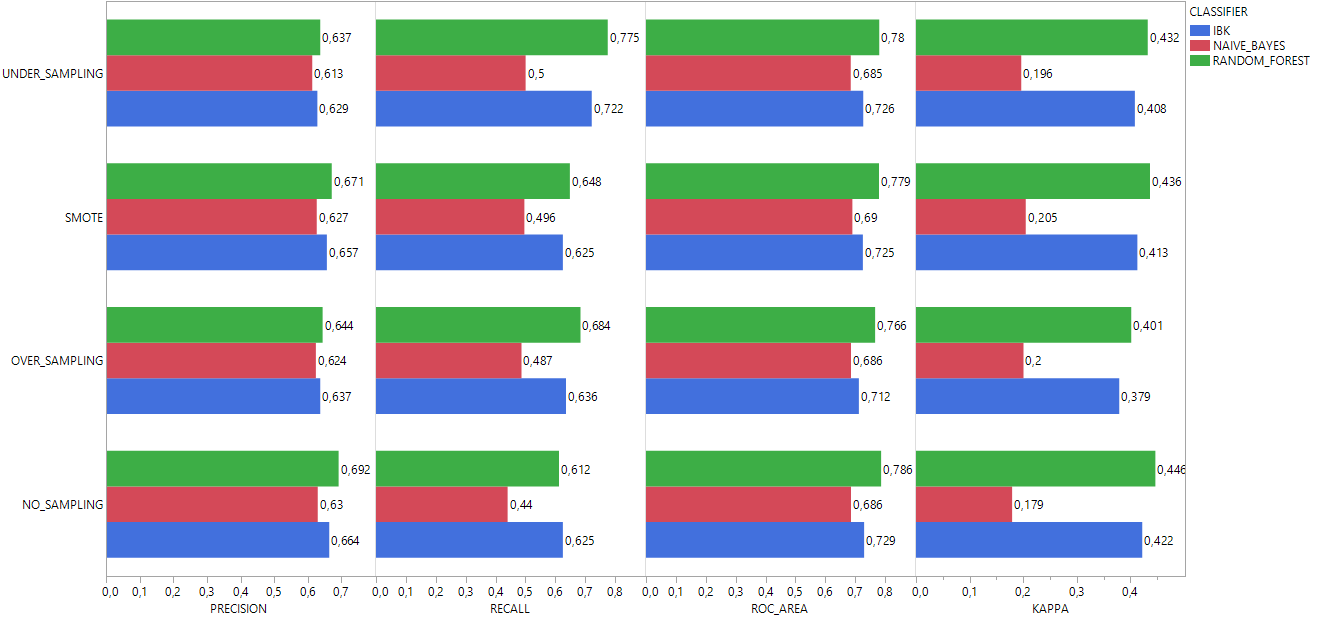
\includegraphics[width=\linewidth]{1 - BOOKKEEPER - SamplingNoFeatureSelection}
  \caption{System Architecture}
  \label{fig:BOOKKEEPER:SamplingNoFeatureSelection}
\end{figure*}







\bibliographystyle{ACM-Reference-Format}
\bibliography{bib}


\end{document}
\endinput


